\chapter{Results}
\section{Implementation and compatibility checks}
The evaluated package was built from isolated source and passed
\texttt{R CMD check}, with examples, manual, and vignettes skipped.
All thirteen package regression files passed. They cover stored entry
times and fresh-process prediction, input validation and retained-row
alignment, restoration and VIMP, tuning, supported splitting rules,
concordance selection, Brier/AUC reference calculations, validation-outcome
alignment, and partial-dependence normalization.

Separate research-code checks compare the Cox prediction-grid helper with
\texttt{survival::survfit}, test cache invalidation after same-version
R-only and native-only package changes, and check worker provenance and
serial/worker agreement. Numerical reference tests and successful package
checks do not establish every statistical modeling assumption.

All 600 simulation replications independently passed the ordinary versus
zero-entry check. The largest RSF survival-curve difference was exactly
zero in every scenario. The largest Cox difference was below
$4\times10^{-14}$. All saved scalar scores were finite and all six result
objects recorded the same package fingerprints. These results replace the
earlier ten-replication summaries as the numerical basis of this draft.

\section{Survival-curve accuracy}
% Generated from the completed 100-replication run; do not edit by hand.
\begin{table}[htbp]
\centering\small
\setlength{\tabcolsep}{4pt}
\begin{tabular}{clrrrrr}
\toprule
Scenario & Model & Entry-blind & Entry-aware & Gain & MCSE & Reduction \\
\midrule
1 & Cox & 0.1110 & 0.0096 & 0.1014 & 0.00042 & 91.39\% \\
1 & RSF & 0.1130 & 0.0384 & 0.0746 & 0.00032 & 66.01\% \\
2 & Cox & 0.1227 & 0.1023 & 0.0205 & 0.00063 & 16.66\% \\
2 & RSF & 0.0946 & 0.0603 & 0.0343 & 0.00030 & 36.23\% \\
3 & Cox & 0.1000 & 0.0185 & 0.0816 & 0.00050 & 81.53\% \\
3 & RSF & 0.1031 & 0.0656 & 0.0376 & 0.00024 & 36.42\% \\
4 & Cox & 0.1511 & 0.0811 & 0.0699 & 0.00096 & 46.30\% \\
4 & RSF & 0.1339 & 0.0784 & 0.0555 & 0.00024 & 41.45\% \\
5 & Cox & 0.2002 & 0.1512 & 0.0490 & 0.00100 & 24.46\% \\
5 & RSF & 0.1297 & 0.0895 & 0.0403 & 0.00031 & 31.05\% \\
6 & Cox & 0.1708 & 0.0881 & 0.0827 & 0.00087 & 48.43\% \\
6 & RSF & 0.1430 & 0.0799 & 0.0631 & 0.00034 & 44.11\% \\
\bottomrule
\end{tabular}
\caption{Mean absolute survival-curve error (MAD). Gain is mean entry-blind minus entry-aware error; positive values favor entry-aware fitting. MCSE is the Monte Carlo standard error of the paired mean gain. Reduction is the gain divided by mean entry-blind error. There are \SimReplications{} replications per scenario.}
\label{tab:mad}
\end{table}

Entry-aware fitting lowered mean truth-based curve error for both model
families in all six scenarios. Relative MAD reductions were
16.66--91.39\% for Cox and 31.05--66.01\% for RSF. Every RSF replication
improved on this measure. Cox improved in all replications except one in
Scenario 2, giving 599 improvements out of 600 Cox comparisons.
Table~\ref{tab:mad} reports absolute paired gains and their MCSEs rather
than relying on percentage changes alone.

\begin{figure}[htbp]
\centering
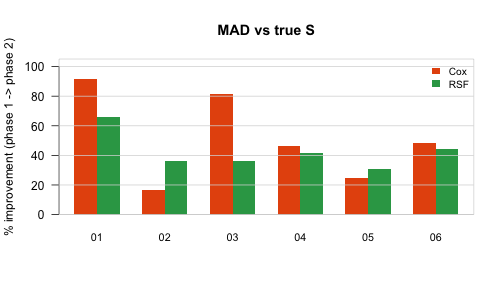
\includegraphics[width=0.95\textwidth]{figures/mad-improvement.png}
\caption{Relative reduction in truth-based MAD after supplying entry times.
Positive values indicate lower error. The figure summarizes 100 paired
replications per scenario; Table~\ref{tab:mad} gives absolute values and
Monte Carlo uncertainty.}
\label{fig:mad}
\end{figure}

For a fixed node, including not-yet-entered subjects inflates the risk
denominator and reduces its event-to-risk hazard increment. Correcting
entry can therefore change the level of a survival curve substantially.
Forest splits and node memberships may also change, so this fixed-node
argument does not determine the final empirical effect by itself.

\section{Outcome-based scores and the mixed concordance finding}
% Generated from the completed run; percentage changes are on error scales.
\begin{table}[htbp]
\centering\small
\setlength{\tabcolsep}{3pt}
\begin{tabular}{crrrrrrrr}
\toprule
 & \multicolumn{2}{c}{MAD} & \multicolumn{2}{c}{Concordance error} & \multicolumn{2}{c}{CRPS} & \multicolumn{2}{c}{AUC error} \\
\cmidrule(lr){2-3}\cmidrule(lr){4-5}\cmidrule(lr){6-7}\cmidrule(lr){8-9}
Scenario & Cox & RSF & Cox & RSF & Cox & RSF & Cox & RSF \\
\midrule
1 & 91.39\% & 66.01\% & 0.03\% & -0.38\% & 5.96\% & 5.48\% & 0.95\% & 1.45\% \\
2 & 16.66\% & 36.23\% & 0.01\% & -1.03\% & 3.84\% & 2.93\% & 0.58\% & 0.30\% \\
3 & 81.53\% & 36.42\% & 0.03\% & -0.02\% & 3.29\% & 1.74\% & 1.42\% & 1.20\% \\
4 & 46.30\% & 41.45\% & 0.03\% & 0.04\% & 4.20\% & 2.51\% & 1.51\% & 1.96\% \\
5 & 24.46\% & 31.05\% & 0.15\% & 0.46\% & 4.20\% & 2.49\% & 1.32\% & 1.45\% \\
6 & 48.43\% & 44.11\% & 0.27\% & 0.66\% & 7.00\% & 4.29\% & 1.02\% & 2.45\% \\
\bottomrule
\end{tabular}
\caption{Percentage reduction in mean error after supplying entry times, $100(\overline E_0-\overline E_L)/\overline E_0$. Positive values favor entry-aware fitting; negative values indicate a higher error. Concordance and AUC columns use $1-C$ and $1-\overline{\mathrm{AUC}}$, respectively. These are relative error changes, not percentage-point changes in C or AUC.}
\label{tab:metric-reductions}
\end{table}

Entered-cohort CRPS and time-averaged AUC error decreased in both model
families in all six scenarios. CRPS reductions ranged from 3.29--7.00\%
for Cox and 1.74--5.48\% for RSF. AUC-error reductions were smaller:
0.58--1.51\% for Cox and 0.30--2.45\% for RSF.
These statements concern the specified entered-cohort scores under the
pooled censoring model, not source-population prediction error.

Concordance changes were smaller and did not uniformly favor entry-aware
RSF. RSF concordance error increased by 0.38\% and 1.03\% in Scenarios 1
and 2, respectively. In Scenario 2, error rose from 0.240740 to 0.243223;
all 100 paired replications showed deterioration on this measure.
The small RSF changes in Scenarios 3 and 4 have descriptive paired
normal-approximation intervals that include zero. Scenarios 5 and 6
show lower RSF concordance error. Absolute means, paired gains, and MCSEs
for all three outcome-based scores appear in the appendix.

\begin{figure}[htbp]
\centering
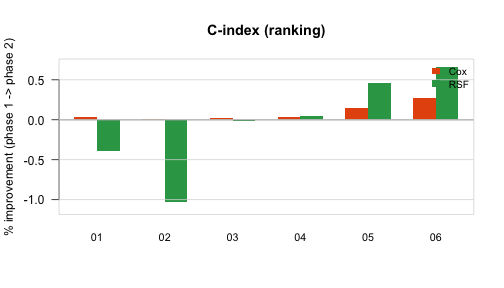
\includegraphics[width=0.95\textwidth]{figures/concordance-improvement.png}
\caption{Relative reduction in entry-aware concordance error.
Negative RSF values show the observed deterioration in some scenarios.
These are relative changes in error, not percentage-point changes in C.}
\label{fig:concordance}
\end{figure}

Improved curve accuracy can coexist with little change or a deterioration
in ranking. The concordance marker sums raw survival-curve event risks;
the AUC marker conditions on each subject's entry. The metrics also use
different time and subject comparisons. Their empirical differences
therefore require interpretation, rather than an expectation that every
metric must move in the same direction.

\section{Historical results and reproducibility}
The completed study is tied to package commit \RunCommit{} and preserved
input files. Its package fingerprints, run configuration, checkpoints,
and generated summary tables are saved with the isolated run.
Historical result objects lack this package provenance. The refresh
includes a corrected Cox grid lookup, scoring and prediction fixes, and
upstream censoring/RNG changes. Differences from historical numbers
cannot be assigned to a single fix. The tables and figures in this draft
are generated from the refreshed results, not from the original saved
ten-replication files.
